\documentclass[11pt,a4paper]{article}

\usepackage[margin=2.4cm]{geometry}
\usepackage{amsmath,amssymb}
\usepackage{graphicx}
\usepackage{booktabs}
\usepackage{hyperref}
\usepackage{caption}
\usepackage{float}
\usepackage{xcolor}
\usepackage{listings}
\usepackage{tcolorbox}

\graphicspath{{../figures/}}
\hypersetup{colorlinks=true, linkcolor=blue, citecolor=blue, urlcolor=blue}

% ---- code listing style -------------------------------------------------
\definecolor{codebg}{RGB}{247,247,250}
\definecolor{codekw}{RGB}{0,60,160}
\definecolor{codestr}{RGB}{150,60,0}
\definecolor{codecom}{RGB}{90,120,90}
\lstset{
  language=Python,
  basicstyle=\ttfamily\footnotesize,
  keywordstyle=\color{codekw}\bfseries,
  stringstyle=\color{codestr},
  commentstyle=\color{codecom}\itshape,
  backgroundcolor=\color{codebg},
  frame=single, framerule=0.3pt, rulecolor=\color{gray!40},
  breaklines=true, showstringspaces=false,
  aboveskip=0.9em, belowskip=0.9em, columns=fullflexible,
}

% ---- "key idea" box -----------------------------------------------------
\newtcolorbox{keyidea}{colback=blue!4!white, colframe=blue!45!black,
  title=Key idea, fonttitle=\bfseries, left=2mm, right=2mm, top=1mm, bottom=1mm}

\title{Strong Lens Inference, Explained From Zero\\[0.5em]
\large A complete beginner's guide to the project --- the physics, the statistics,\\
the code, and how to read every plot}
\author{Sayed Atique Newaz \and Noureen Alam Meem \and Mashuk Khan}
\date{July 2026}

\begin{document}
\maketitle

\begin{abstract}
\noindent This document explains the entire project assuming \emph{no} prior
knowledge: not of astronomy, not of Bayesian statistics, not of neural networks.
It walks through what gravitational lensing is, what problem we are solving, how
the code solves it (with the important pieces of source code shown and explained
line by line), and then --- plot by plot --- what each figure in the project means,
how to read it, and what ours actually shows. It accompanies the formal project
report (\texttt{report/report.pdf}); read this one first.
\end{abstract}

\tableofcontents
\newpage

% =========================================================================
\section{The big picture: what are we even doing?}

Imagine you find a photograph of a strange circle of light in the sky. You are
told: \emph{a massive galaxy bent the light of another galaxy behind it, and this
ring is the result}. The photograph is blurry and noisy. Your task:

\begin{center}
\emph{From this one picture, work out the physical properties of the galaxy that
bent the light --- how heavy it is, how squashed its shape is, where exactly the
background galaxy sits behind it --- and say how sure you are about each number.}
\end{center}

That is the whole project. Three things make it hard:

\begin{enumerate}
  \item \textbf{The physics only runs forward.} Given the galaxy's properties, we
  can compute the picture (that is a simulation). But there is no formula that
  takes the picture and returns the properties.
  \item \textbf{The picture is noisy.} A real detector adds random noise, so even
  the forward direction is not exact --- many slightly different pictures could
  come from the same galaxy.
  \item \textbf{We need error bars, not just numbers.} ``The mass is 1.2'' is
  much less useful than ``the mass is $1.20 \pm 0.01$''. Science runs on
  uncertainties.
\end{enumerate}

\begin{keyidea}
We solve it by \textbf{simulation-based inference (SBI)}: simulate tens of
thousands of fake galaxies and their pictures, then train a neural network to go
\emph{backwards} --- from picture to a full probability distribution over the
galaxy's properties. Train once, then answer for any new picture in milliseconds.
\end{keyidea}

% =========================================================================
\section{The physics: gravitational lensing in plain words}

\subsection{Mass bends light}

Einstein's general relativity says mass curves space, and light follows that
curvature. A galaxy is heavy enough ($\sim$$10^{11}$ times the mass of the Sun)
that light passing near it gets visibly deflected --- the galaxy acts like a huge,
slightly imperfect glass lens floating in space.

\subsection{What we see depends on alignment}

Put a distant ``source'' galaxy almost exactly behind a nearby ``lens'' galaxy:

\begin{itemize}
  \item \textbf{Perfect alignment} $\rightarrow$ the source's light is smeared
  into a complete circle: an \emph{Einstein ring}.
  \item \textbf{Slight offset} $\rightarrow$ the ring breaks into stretched
  \emph{arcs}, or the source appears \emph{multiple times} in one image.
\end{itemize}

Crucially, the distortion is not random --- it encodes the lens:

\begin{center}
\begin{tabular}{ll}
\toprule
\textbf{What you measure in the image} & \textbf{What it tells you} \\
\midrule
Radius of the ring/arcs & The mass of the lens (Einstein radius $\theta_E$) \\
How the arcs are squashed & The lens galaxy's shape ($e_1, e_2$) \\
An extra overall stretch & Gravity of \emph{neighbouring} structures ($\gamma_1, \gamma_2$) \\
Where the arcs sit & Where the source really is ($x_s, y_s$) \\
How thick the arcs are & How big the source is ($R_s$) \\
\bottomrule
\end{tabular}
\end{center}

\subsection{The eight (or nine) numbers we infer}

Bundling those together, our unknown parameter vector is
\[
\boldsymbol\theta = (\underbrace{\theta_E}_{\text{mass}},\;
\underbrace{e_1, e_2}_{\text{lens shape}},\;
\underbrace{\gamma_1, \gamma_2}_{\text{external tug}},\;
\underbrace{x_s, y_s}_{\text{source position}},\;
\underbrace{R_s}_{\text{source size}})
\;\;[\,+\ \kappa\,].
\]

The optional ninth number $\kappa$ (``external convergence'') is a thin uniform
sheet of extra mass in front of everything. It matters for a special reason
explained in Section~\ref{sec:msd}: physics \emph{proves} it cannot be measured
from a single image, so it lets us test whether our method is honest about what
it cannot know.

% =========================================================================
\section{The statistics: Bayesian inference from zero}

\subsection{Uncertainty as probability}

Bayesian inference is bookkeeping for beliefs. Before seeing data you have a
\textbf{prior} $p(\boldsymbol\theta)$: which parameter values are plausible at
all. The simulator defines the \textbf{likelihood}
$p(\mathbf{x} \mid \boldsymbol\theta)$: how probable is the observed image
$\mathbf{x}$ if the truth were $\boldsymbol\theta$. Bayes' rule combines them
into the \textbf{posterior} --- what you believe \emph{after} seeing the image:
\[
\underbrace{p(\boldsymbol\theta \mid \mathbf{x})}_{\text{posterior}}
\;=\;
\frac{\overbrace{p(\mathbf{x} \mid \boldsymbol\theta)}^{\text{likelihood}}
      \;\overbrace{p(\boldsymbol\theta)}^{\text{prior}}}
     {p(\mathbf{x})}.
\]

The posterior is the complete answer to our task: for every parameter it gives a
best value \emph{and} an uncertainty \emph{and} all correlations between
parameters (``if the mass is a bit higher, the source must be a bit smaller'').

\subsection{Why the textbook route fails here}

To use Bayes' rule directly you must be able to \emph{evaluate} the likelihood as
a formula. Our image is produced by ray-tracing light through a lens model,
blurring with the telescope optics, and adding two kinds of noise. There is no
closed-form expression for $p(\mathbf{x} \mid \boldsymbol\theta)$ you could type
into a computer. Classical tools (like MCMC) that need that formula are stuck ---
or need expensive approximations, hours per lens.

\subsection{The SBI trick: learn the inverse from examples}

We \emph{can} sample from the likelihood --- that is literally what the simulator
does. So:

\begin{enumerate}
  \item Draw a random $\boldsymbol\theta^{(i)}$ from the prior.
  \item Simulate its noisy image $\mathbf{x}^{(i)}$.
  \item Repeat 50{,}000 times $\rightarrow$ a big table of
  $(\boldsymbol\theta, \mathbf{x})$ pairs.
  \item Train a neural network so that, shown $\mathbf{x}$, it outputs a
  distribution close to the true $p(\boldsymbol\theta \mid \mathbf{x})$.
\end{enumerate}

\begin{keyidea}
The network never sees a formula for the likelihood --- only examples. All the
physics enters through the simulator. This is why the method is called
\emph{simulation-based} (or \emph{likelihood-free}) inference, and because one
training pays for all future images, it is \emph{amortized}.
\end{keyidea}

% =========================================================================
\section{The code, part 1: simulating fake universes}

Everything configurable lives in one file, \texttt{src/config.py}. The pipeline
is run from the command line:

\begin{lstlisting}
python main.py generate   # simulate the dataset  (CPU, ~1 minute)
python main.py train      # train the network     (GPU, ~2 hours)
python main.py evaluate   # produce all the plots in figures/
\end{lstlisting}

\subsection{Drawing random galaxies: the prior}

The prior ranges are plain numbers in \texttt{config.py} --- every one chosen so
the simulated system is a physically valid, visibly lensed galaxy:

\begin{lstlisting}
PRIOR = {
    "theta_E": (0.7, 1.6),   # Einstein radius: keeps the ring inside the image
    "q":       (0.6, 1.0),   # lens axis ratio -> converted to (e1, e2)
    "phi":     (0.0, 3.14),  # lens orientation angle
    "gamma_ext": (0.0, 0.08),# external shear strength (it is always weak)
    "phi_ext": (0.0, 3.14),  # external shear direction
    "x_s": (-0.3, 0.3),      # source position
    "y_s": (-0.3, 0.3),
    "R_s": (0.05, 0.25),     # source size (arc thickness)
    "kappa": (0.0, 0.20),    # mass sheet -- only in the 9-parameter version
}
\end{lstlisting}

Notice we do \emph{not} draw $e_1, e_2$ directly. We draw a squashing factor $q$
and an angle $\phi$ --- quantities with clear physical meaning --- and convert
(\texttt{src/simulator/parameters.py}):

\begin{lstlisting}
def _ellipticity_from_q_phi(q, phi):
    """Axis ratio q + position angle phi -> (e1, e2).
    Guarantees every draw is a valid ellipse (e1^2 + e2^2 < 1)."""
    e = (1.0 - q) / (1.0 + q)
    return e * np.cos(2.0 * phi), e * np.sin(2.0 * phi)
\end{lstlisting}

This tiny function has a visible consequence: the ring-shaped clouds you will see
in the prior plot (Figure~\ref{fig:prior-pairs}) are exactly the geometry this
conversion creates. They are correct by construction, not a bug.

\subsection{From parameters to picture}

The simulator (\texttt{src/simulator/lens\_generator.py}) hands the parameters to
\texttt{lenstronomy}, a standard astrophysics package, which solves the lens
equation --- ``which point of the source does each pixel actually show?'' --- then
blurs the result with the telescope's point-spread function (PSF) and samples it
onto a $64\times64$ pixel grid, exactly like a small telescope camera would.

\subsection{Making it look real: noise}

A real detector adds two kinds of randomness, and we add both
(\texttt{src/simulator/noise.py}):

\begin{lstlisting}
def add_noise(clean_image, rng=None):
    """Gaussian background + Poisson shot noise, exactly like a real CCD."""
    background_noise = image_util.add_background(clean_image,
                                                 sigma_bkd=C.BACKGROUND_RMS)
    poisson_noise    = image_util.add_poisson(clean_image,
                                              exp_time=C.EXP_TIME)
    return clean_image + background_noise + poisson_noise
\end{lstlisting}

\emph{Background noise} is the constant hiss of the sky and the electronics.
\emph{Poisson (shot) noise} exists because light arrives as individual photons:
brighter pixels receive more photons and therefore fluctuate more in absolute
terms. Getting the noise level right mattered enormously: our first datasets were
too faint (peak signal-to-noise $\approx 4$) and the network could not learn the
subtle parameters at all. After a brightness sweep we reached a realistic median
peak SNR of $\approx 16$.

\subsection{The dataset}

50{,}000 training + 2{,}000 validation + 300 test systems are simulated in
parallel on all CPU cores and stored to disk, so training never touches the
simulator again. Figure~\ref{fig:dataset-preview} shows what the network actually
gets as input.

\begin{figure}[H]
\centering
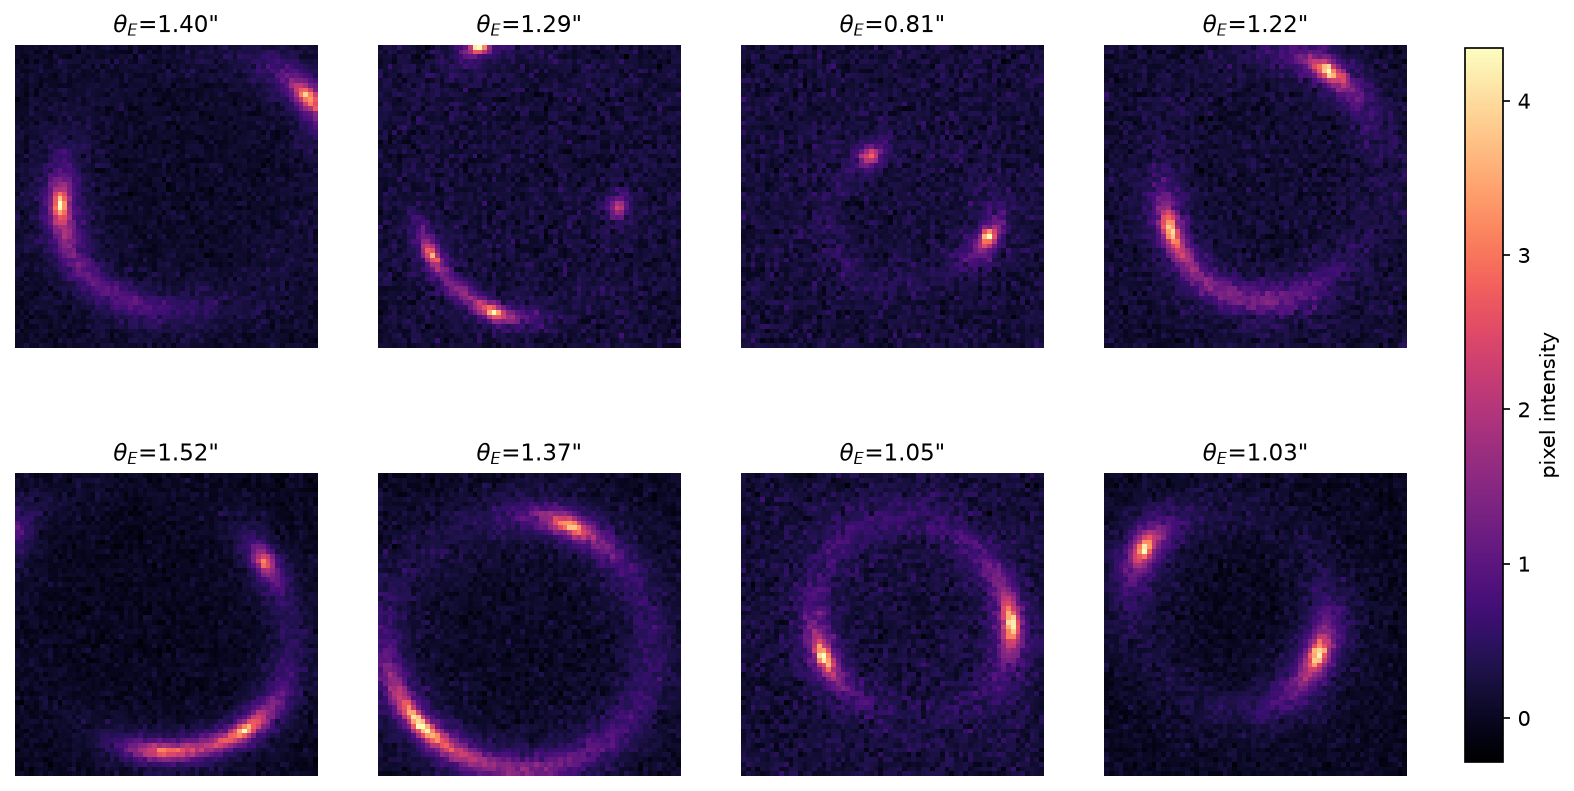
\includegraphics[width=0.85\textwidth]{dataset_preview.png}
\caption{\textbf{Eight training images.} Each panel is one simulated ``telescope
photo'' (with noise) labelled by its true Einstein radius $\theta_E$. Note the
variety: complete rings, broken arcs, thick and thin, centred and offset. This
variety is the point --- the network must learn to read \emph{any} of these.}
\label{fig:dataset-preview}
\end{figure}

\begin{figure}[H]
\centering
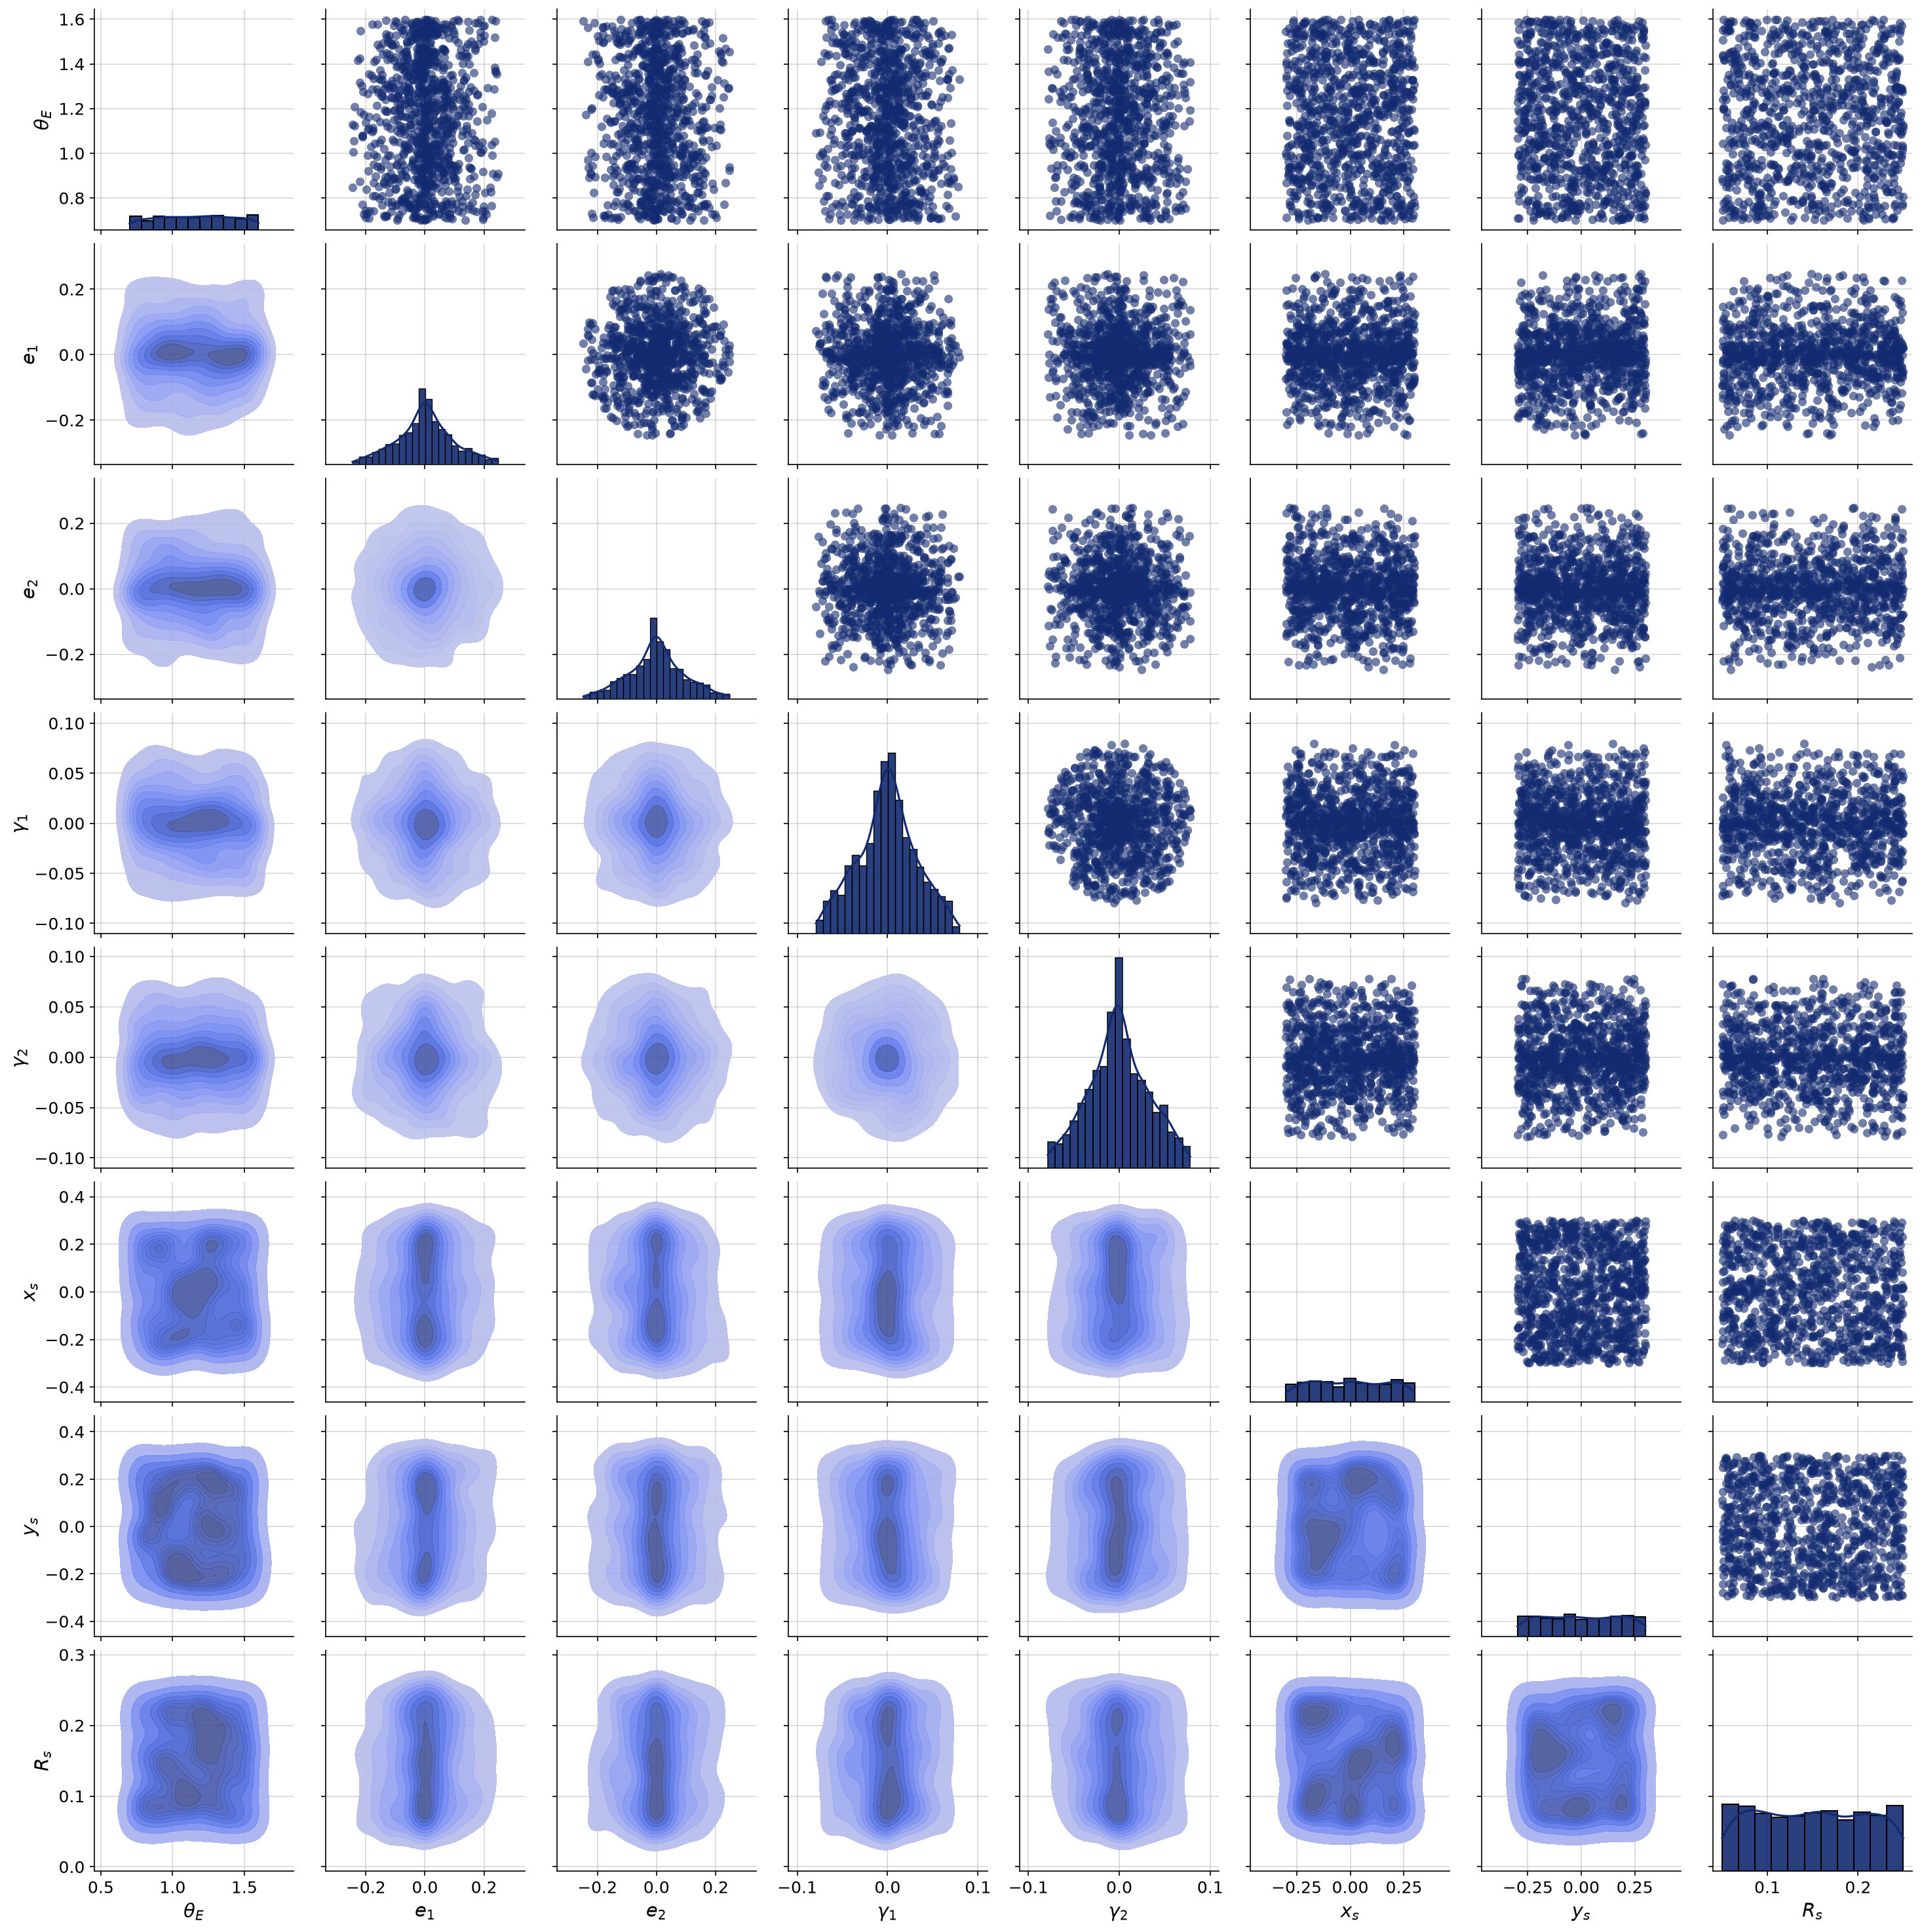
\includegraphics[width=0.88\textwidth]{prior_pairs.png}
\caption{\textbf{The prior, visualized.} Diagonal panels: the distribution of each
parameter across the training set (flat, as designed). Off-diagonal panels: every
pair of parameters plotted against each other. The ring/disc shapes in the
$(e_1,e_2)$ and $(\gamma_1,\gamma_2)$ panels come from drawing (strength, angle)
pairs and converting to Cartesian components --- the code shown above.}
\label{fig:prior-pairs}
\end{figure}

% =========================================================================
\section{The code, part 2: the neural networks}

The posterior estimator is two networks trained together end to end.

\subsection{The summary network: 4096 pixels $\rightarrow$ 48 numbers}

A $64\times64$ image is 4096 numbers, most of them noise. The summary network is
a small \textbf{convolutional neural network (CNN)} --- the standard architecture
for images --- that learns to compress each image into 48 numbers that retain the
information about $\boldsymbol\theta$
(\texttt{src/models/bayesflow\_model.py}):

\begin{lstlisting}
self.net = keras.Sequential([
    layers.Rescaling(1.0 / C.IMAGE_SCALE),        # bring pixels near O(1)

    layers.Conv2D(32, 3, padding="same", activation="relu"),
    layers.Conv2D(32, 3, padding="same", activation="relu"),
    layers.MaxPooling2D(),                         # 64 -> 32 pixels
    layers.BatchNormalization(),

    layers.Conv2D(64, 3, padding="same", activation="relu"),
    layers.Conv2D(64, 3, padding="same", activation="relu"),
    layers.MaxPooling2D(),                         # 32 -> 16
    layers.BatchNormalization(),

    layers.Conv2D(128, 3, padding="same", activation="relu"),
    layers.Conv2D(128, 3, padding="same", activation="relu"),
    layers.MaxPooling2D(),                         # 16 -> 8
    layers.BatchNormalization(),

    layers.GlobalAveragePooling2D(),               # -> 128 numbers
    layers.Dense(128, activation="relu"),
    layers.Dense(summary_dim),                     # -> 48 numbers
])
\end{lstlisting}

How to read this if you have never seen a CNN: each \texttt{Conv2D} layer slides
many small $3\times3$ ``feature detectors'' across the image; early layers learn
to respond to simple things (edges, bright spots), later layers to combinations
of them (arc segments, ring curvature). Each \texttt{MaxPooling2D} halves the
resolution, so by the last block the network is looking at the picture as a whole.
Nobody tells it \emph{which} features matter --- it discovers, during training,
whatever 48 numbers best predict the parameters.

\subsection{The inference network: 48 numbers $\rightarrow$ a full distribution}

The second network is a \textbf{conditional normalizing flow} (a
\emph{coupling flow} of depth 4). The intuition: it is a flexible, invertible,
learnable ``warping machine''. It takes simple random noise (a standard Gaussian)
and warps it --- in a way that depends on the 48-number summary --- into the shape
of the posterior. Because the warp is invertible, the network can both
\emph{evaluate} how probable a given $\boldsymbol\theta$ is and \emph{generate}
new posterior samples cheaply. Sampling 2{,}000 plausible parameter sets for one
image takes milliseconds.

This is what a plain ``CNN that predicts 8 numbers'' could never do: the flow
outputs the entire joint distribution --- widths, asymmetries, and correlations
between parameters --- not just a best guess.

\subsection{Training: what the loss means}

Training (\texttt{src/models/train.py}) shows the networks batches of
$(\boldsymbol\theta, \mathbf{x})$ pairs and adjusts the weights to maximize the
probability the flow assigns to the \emph{true} $\boldsymbol\theta$ of each image
--- equivalently, to minimize the \emph{negative log-posterior density}. If that
loss goes down, the network's distributions are becoming both better centred and
better sized.

\begin{lstlisting}
early_stop = keras.callbacks.EarlyStopping(
    monitor="val_loss", patience=10, restore_best_weights=True)

history = workflow.fit_offline(
    train_data, epochs=C.EPOCHS, batch_size=C.BATCH_SIZE,
    validation_data=val_data, callbacks=[early_stop])
\end{lstlisting}

Two safety mechanisms are visible here. The \emph{validation set} (2{,}000 images
the optimizer never trains on) tells us whether the network is genuinely learning
or just memorizing. \emph{Early stopping} watches that validation loss and halts
training if it stops improving --- a guard against memorization
(``overfitting'').

\begin{figure}[H]
\centering
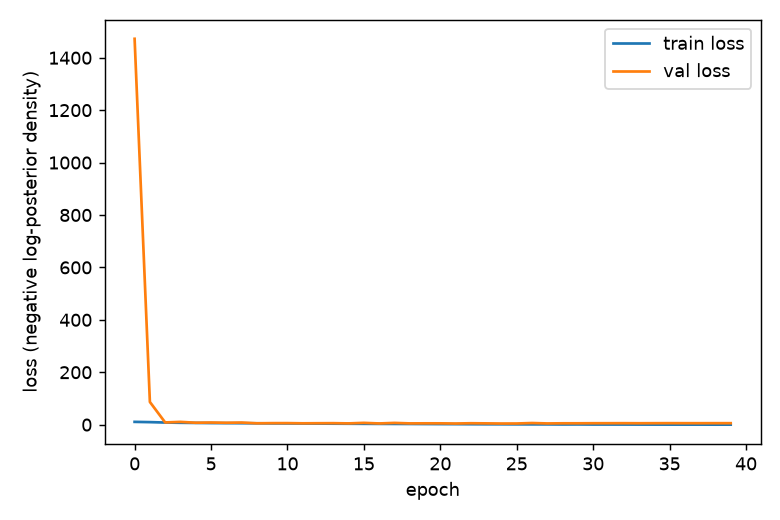
\includegraphics[width=0.8\textwidth]{training_loss.png}
\caption{\textbf{The loss trajectory.} Thin lines: per-epoch loss; thick lines:
moving average. \emph{How to read it:} both curves should fall together. If the
(dashed) validation curve turned upward while the training curve kept falling,
the network would be memorizing --- overfitting. \emph{What ours shows:} both fall
smoothly for all 40 epochs and validation ends \emph{below} training at $-8.05$
--- no overfitting at all; early stopping never had to intervene. (Our early
8{,}000-image pilot \emph{did} overfit; scaling the dataset cured it.)}
\label{fig:loss}
\end{figure}

% =========================================================================
\section{The plots, part 1: does it work? (accuracy)}

All checks below use the 300 \emph{test} systems --- simulated lenses the network
has never seen --- with 2{,}000 posterior samples drawn per system.

\subsection{Parameter recovery: truth vs.\ estimate}

\begin{figure}[H]
\centering
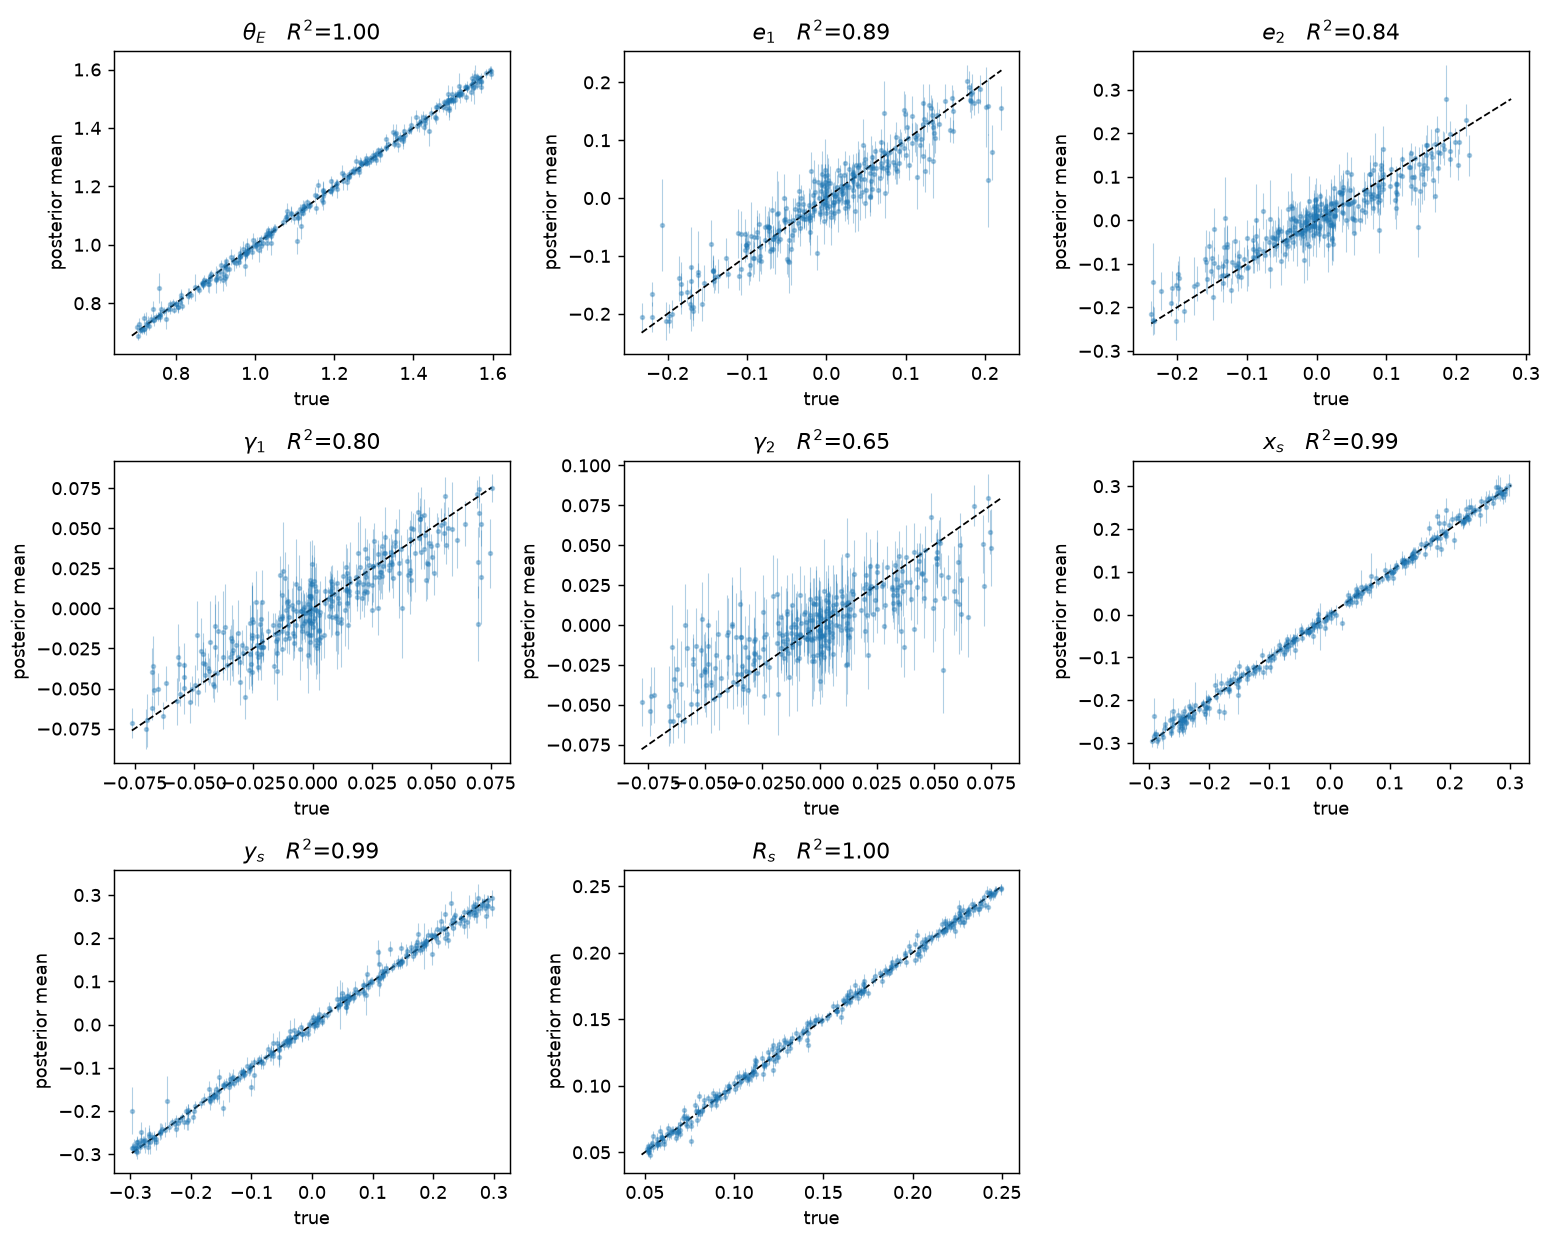
\includegraphics[width=\textwidth]{recovery.png}
\caption{\textbf{Parameter recovery.} One panel per parameter. Horizontal axis:
the true value used to simulate the image. Vertical axis: the network's estimate
(the posterior median), with the posterior spread (MAD) as an error bar. The
dashed diagonal is perfection; $r$ is the correlation between truth and
estimate.}
\label{fig:recovery}
\end{figure}

\textbf{How to read it.} Three things to look at, per panel:
\begin{itemize}
  \item \emph{Do the points follow the diagonal?} If yes, the estimates are
  accurate.
  \item \emph{Is the cloud flat instead?} Then the image does not constrain that
  parameter --- the network falls back towards the prior average (this is honest
  behaviour, not failure).
  \item \emph{Are the error bars the right size?} They should be large exactly
  where the scatter is large.
\end{itemize}

\textbf{What ours shows.} A clean three-tier hierarchy that mirrors the physics:
\begin{center}
\begin{tabular}{llll}
\toprule
Tier & Parameters & $r$ & Why \\
\midrule
Near-perfect & $\theta_E,\ x_s,\ y_s,\ R_s$ & 0.999 & they set ring size/position/thickness \\
Very good & $e_1,\ e_2$ & 0.97 / 0.96 & arc squashing is measurable at SNR 16 \\
Good & $\gamma_1,\ \gamma_2$ & 0.93 / 0.90 & shear is tiny ($\le 0.08$) and subtle \\
\bottomrule
\end{tabular}
\end{center}
The shear error bars are visibly the widest --- the network \emph{knows} shear is
its weakest measurement, which is exactly what we want from a posterior.

\subsection{The closed loop: posterior predictive check}

\begin{figure}[H]
\centering
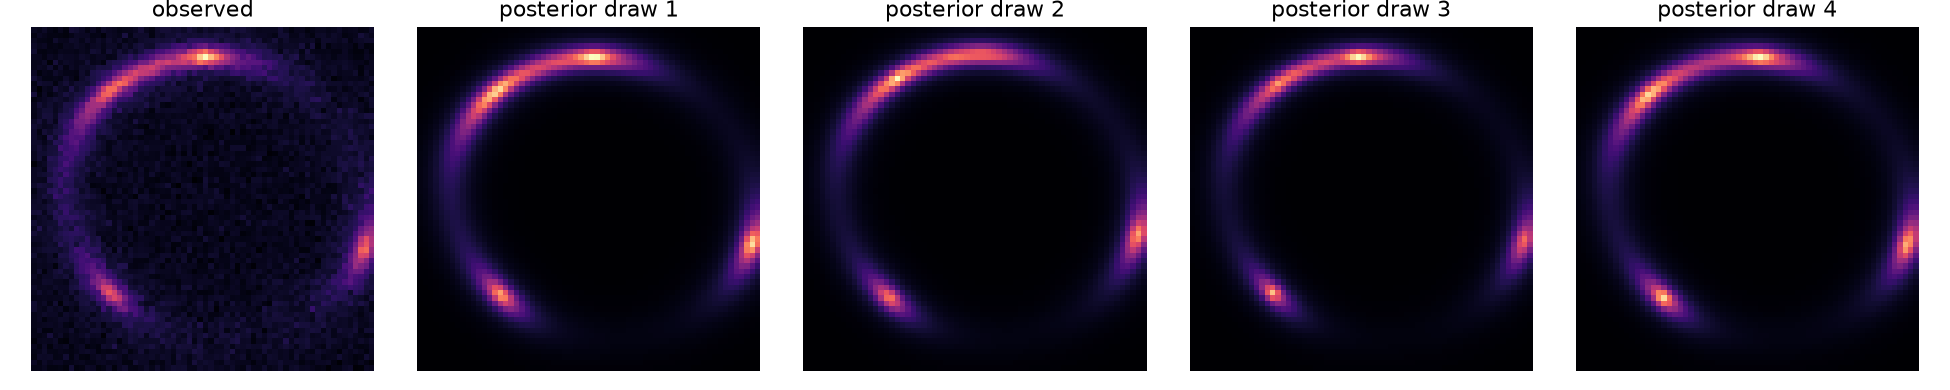
\includegraphics[width=\textwidth]{posterior_predictive.png}
\caption{\textbf{Posterior predictive check.} Leftmost: one observed (noisy) test
image. The other four panels: we drew four independent parameter sets from the
network's posterior for that image and re-simulated each one (noise-free).}
\label{fig:ppc}
\end{figure}

\textbf{How to read it.} If the posterior is centred on the right parameters,
pushing its samples back through the simulator must reproduce the observation.
Differences \emph{between} the four re-simulations visualize the remaining
uncertainty. \textbf{What ours shows:} ring radius, the bright knots, and the
light distribution are all reproduced; the draws differ only in fine knot
brightness --- precisely the detail that the noise genuinely erases. The network
reconstructs what is knowable and stays uncertain about what is not.

% =========================================================================
\section{The plots, part 2: can we trust the error bars? (calibration)}

Accuracy is not enough. A method that says ``$\theta_E = 1.20 \pm 0.001$'' when
the truth is regularly $1.25$ is \emph{worse} than useless --- it is confidently
wrong. So we test the error bars themselves.

\subsection{Simulation-based calibration (SBC)}

The logic, in dice terms: if a weather service's ``70\% chance of rain'' is
honest, it must rain on 70\% of such days. Analogously, the true parameter must
fall in the central 50\% of the posterior 50\% of the time, in the central 90\%
of it 90\% of the time, and so on. Since we \emph{simulated} the test systems, we
know every truth and can check this directly: for each system, compute the
\emph{rank} of the truth within the 2{,}000 posterior samples. Honest posteriors
$\Rightarrow$ ranks uniformly distributed between 0 and 1.

\begin{figure}[H]
\centering
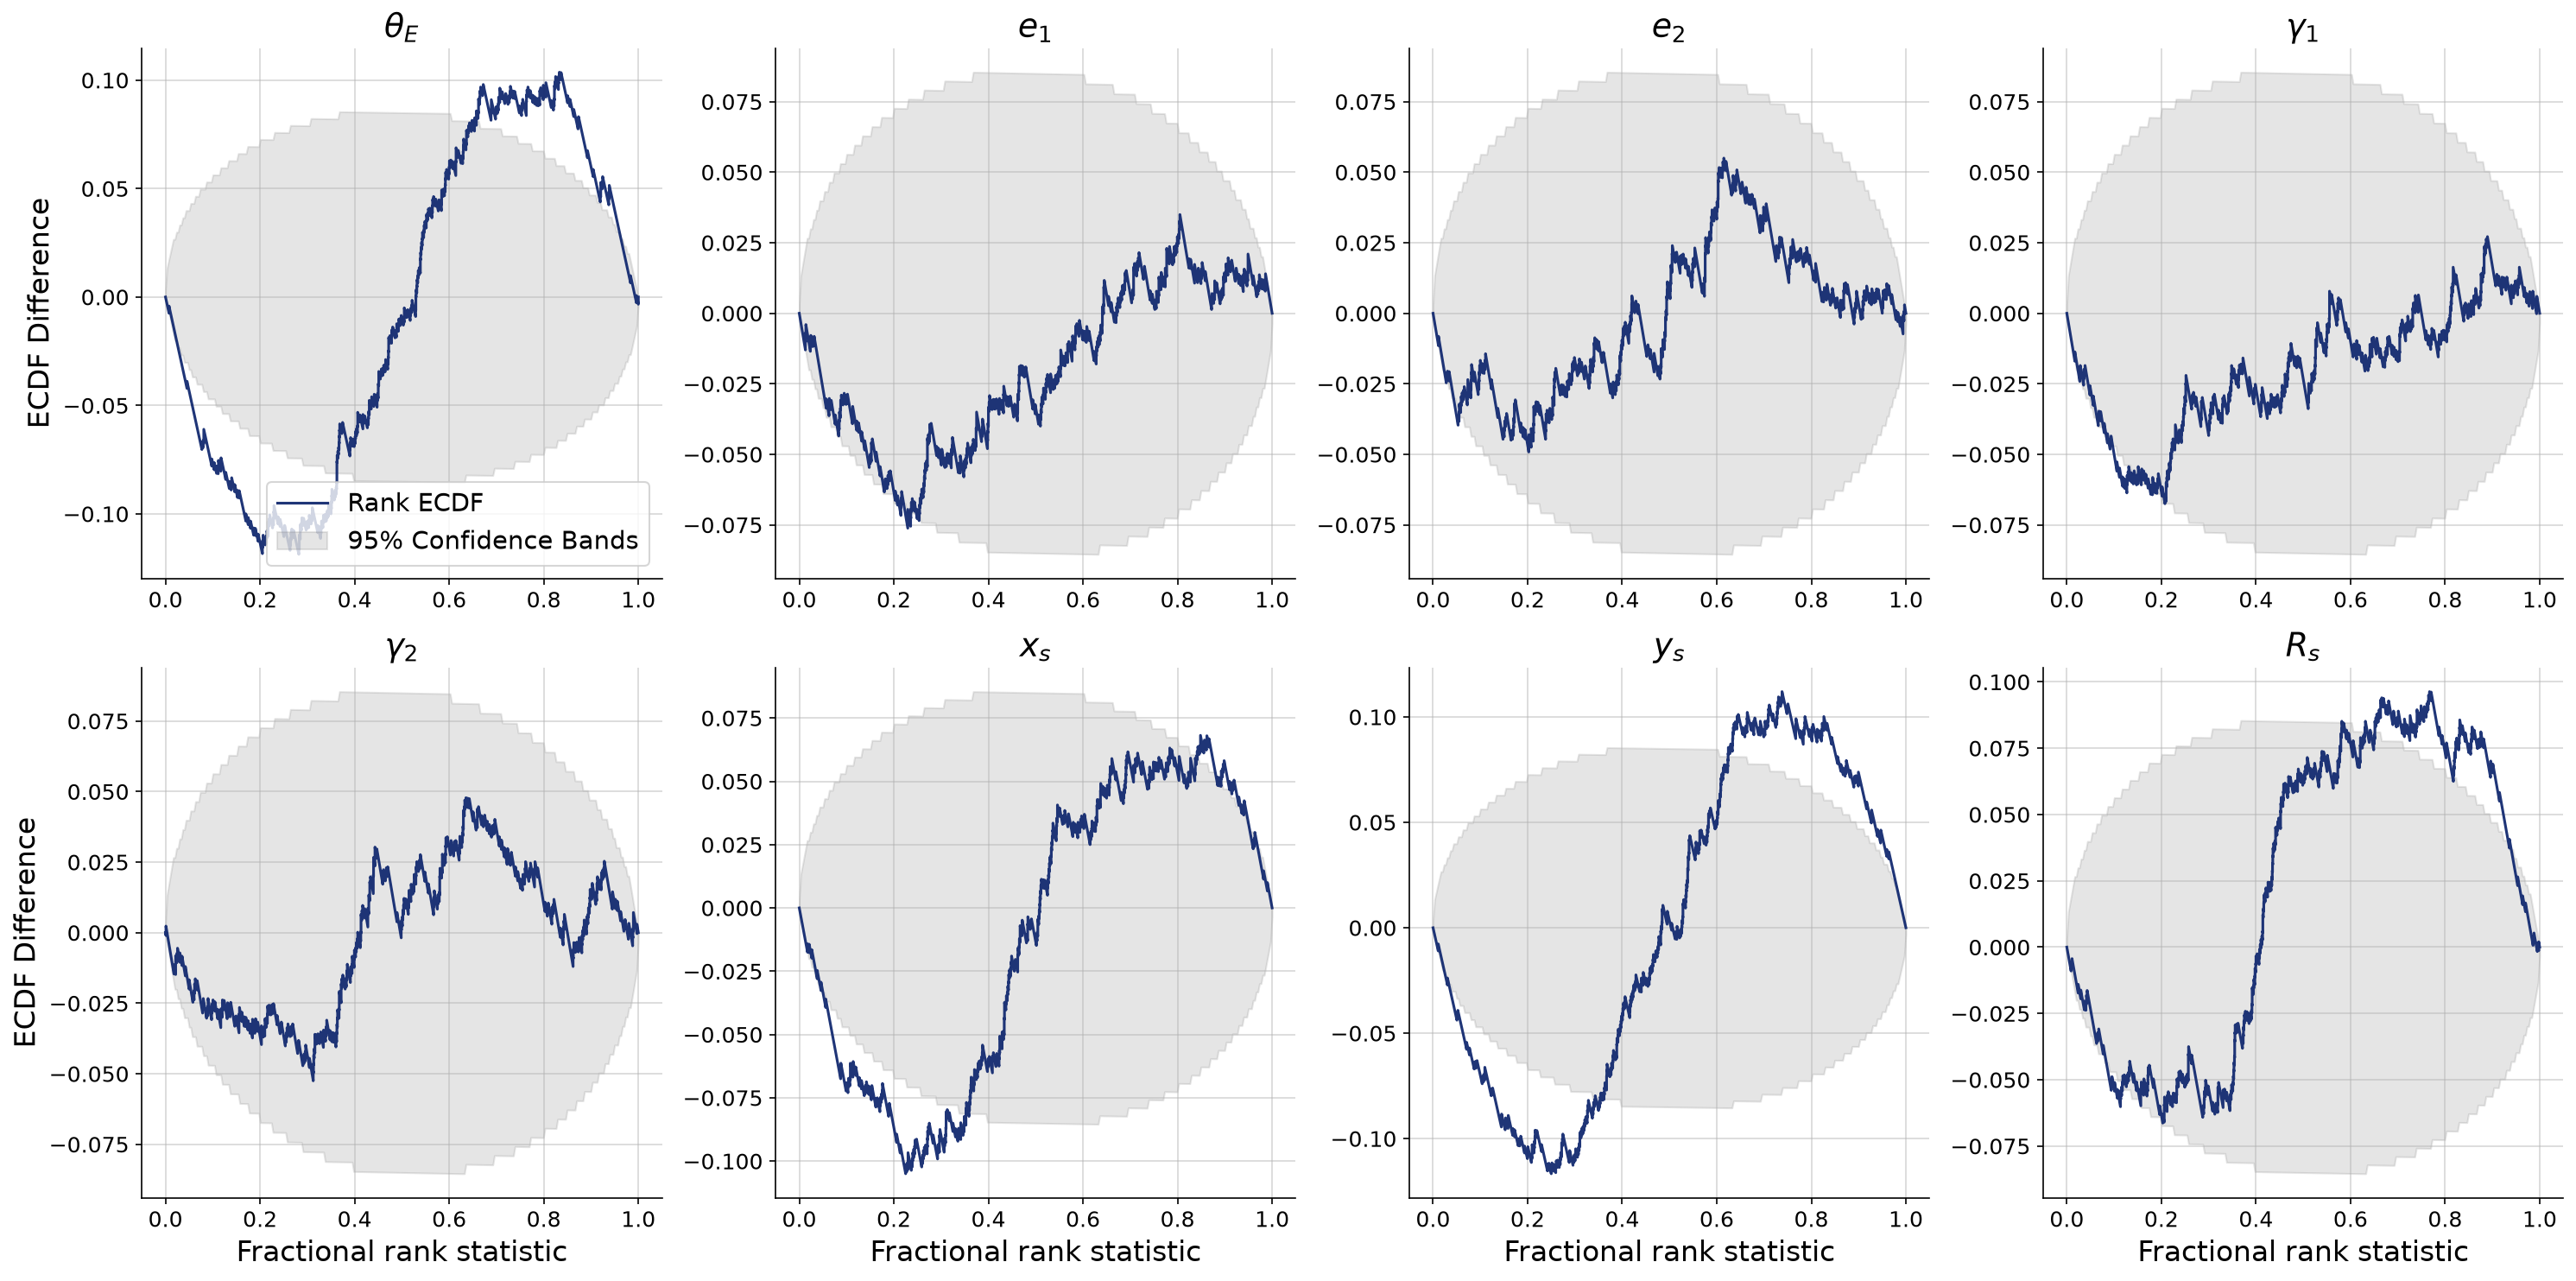
\includegraphics[width=\textwidth]{calibration_ecdf.png}
\caption{\textbf{SBC rank-ECDF difference.} For each parameter, the blue curve is
the difference between the observed distribution of ranks and perfect
uniformity; the grey ellipse is the band inside which an honest method stays 95\%
of the time.}
\label{fig:sbc}
\end{figure}

\textbf{How to read it.} The shape of the excursion is a diagnosis:
\begin{itemize}
  \item \emph{Inside the band} $\rightarrow$ calibrated. Trust the error bars.
  \item \emph{Dip-then-peak S-shape} (too few extreme ranks, too many central
  ones) $\rightarrow$ posteriors too \emph{wide} $\rightarrow$
  \textbf{underconfident}. Conservative; the safe failure.
  \item \emph{The mirror image} (rank pile-up at the extremes) $\rightarrow$
  posteriors too \emph{narrow} $\rightarrow$ \textbf{overconfident}. The dangerous
  failure.
\end{itemize}

\textbf{What ours shows.} Ellipticity and shear: inside the band --- calibrated.
The four best-measured parameters ($\theta_E, x_s, y_s, R_s$): a mild S-shape
outside the band --- their error bars are slightly too wide. Two important
qualifications: (1) this is the harmless direction --- our intervals never
\emph{overclaim}; (2) the shape is \emph{identical} at 20{,}000 and 50{,}000
training images, so more data does not fix it --- it is a limitation of the
network's capacity (the 48-number summary / depth-4 flow), and we know exactly
which knob to turn next. Finding, quantifying, and diagnosing this is what
calibration tests are \emph{for}.

\subsection{Contraction and z-scores: how much did we learn, and is it biased?}

\begin{figure}[H]
\centering
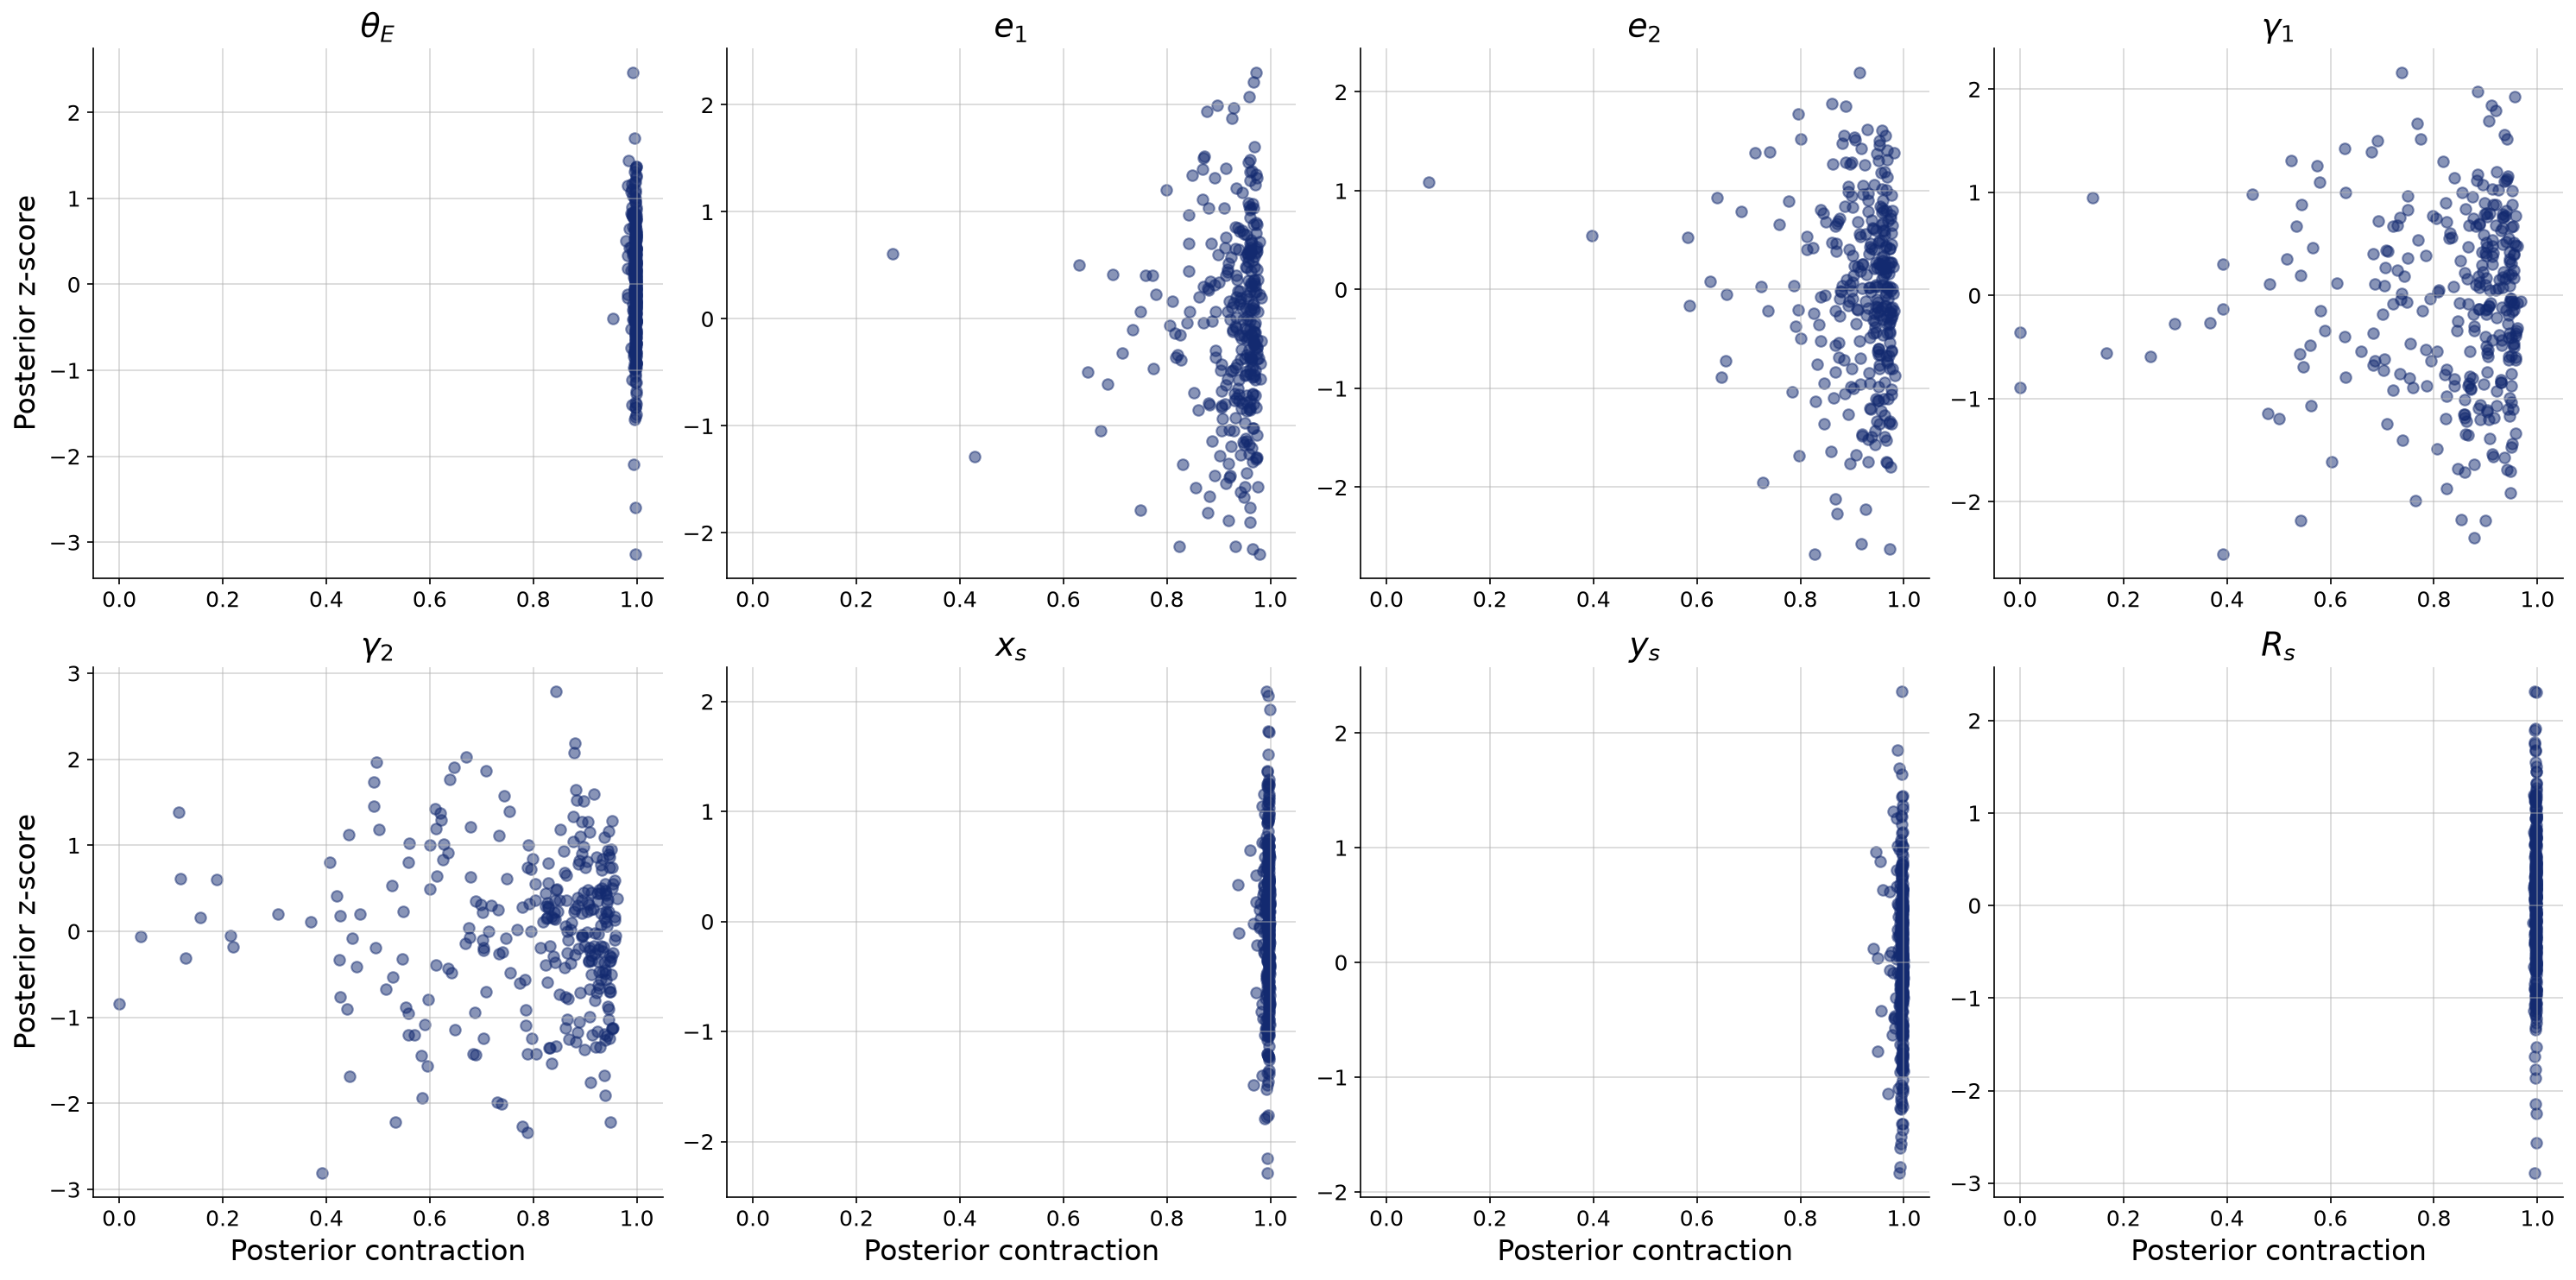
\includegraphics[width=\textwidth]{contraction.png}
\caption{\textbf{Posterior z-score vs.\ posterior contraction}, one dot per test
system. Horizontal axis: contraction $= 1 - \sigma^2_{\rm posterior} /
\sigma^2_{\rm prior}$ (0 = the image taught us nothing; 1 = it removed all prior
uncertainty). Vertical axis: $(\text{posterior mean} - \text{truth}) /
\sigma_{\rm posterior}$, i.e.\ the error measured in units of the claimed
uncertainty.}
\label{fig:contraction}
\end{figure}

\textbf{How to read it.} The ideal is the upper-right ``funnel'': contraction
near 1 and z-scores spread tightly around 0 (roughly within $\pm 2$, like a
standard normal). Low contraction is acceptable \emph{if} z-scores remain centred
--- that just means ``the image contains little information about this parameter,
and the network says so honestly''. \textbf{What ours shows:} the
morphology-dominant parameters sit at contraction $\approx 1$ with centred
z-scores --- maximal, unbiased information gain. Ellipticity and shear reach
intermediate contraction with z-scores still centred: less information, honestly
reported, no bias.

\subsection{One complete inference, visualized}

\begin{figure}[H]
\centering
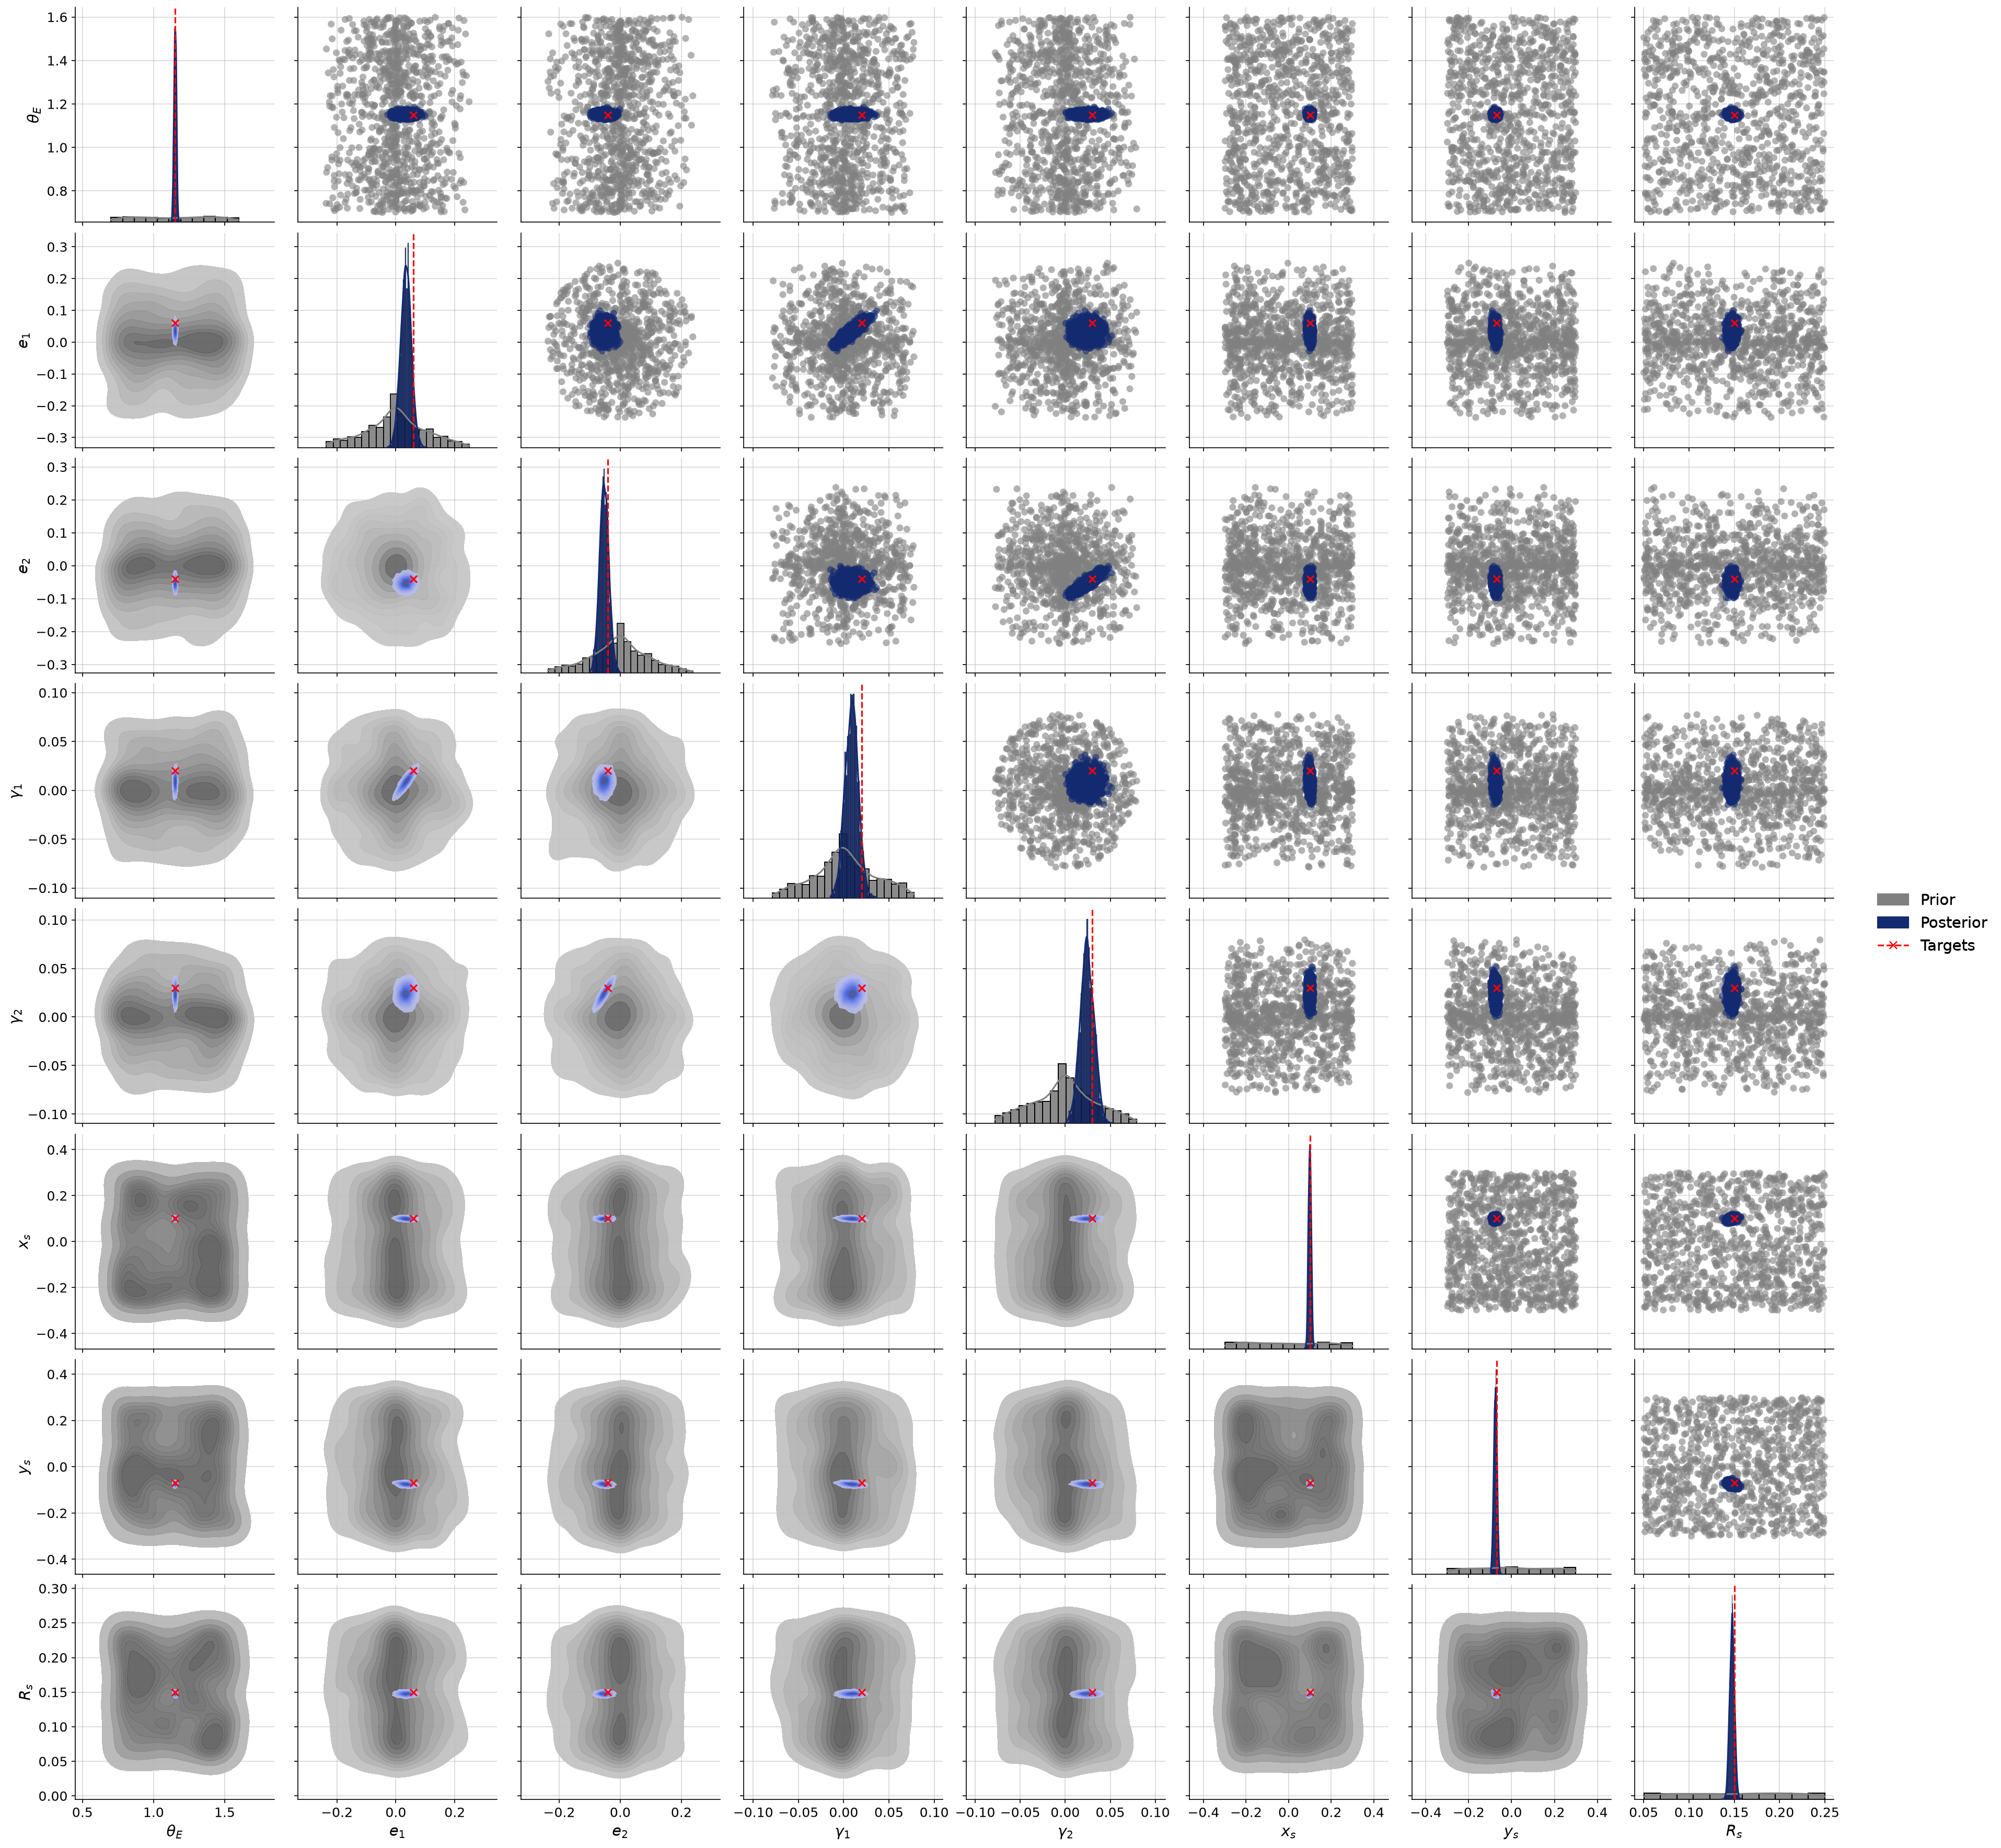
\includegraphics[width=0.95\textwidth]{inference_pairs.png}
\caption{\textbf{The corner plot for one ``observed'' system.} Grey: the prior
(what we believed before looking). Blue: 2{,}000 posterior samples (after looking
at one image). Red: the true values used to simulate that image. Diagonal:
per-parameter distributions; off-diagonal: every pair of parameters jointly.}
\label{fig:corner}
\end{figure}

\textbf{How to read it.} Three checks: the blue blob should be much smaller than
the grey cloud (we learned a lot), it should contain the red marker (we learned
the \emph{right} thing), and its tilts reveal parameter correlations (``these two
trade off against each other''). \textbf{What ours shows:} dramatic contraction
onto the truth --- e.g.\ $\theta_E = 1.152 \pm 0.008$ against a truth of $1.150$
--- with the widest surviving spread in the shear components, and clearly tilted
ellipses showing the network reports \emph{joint} structure, not just eight
separate error bars.

% =========================================================================
\section{The plots, part 3: the physics exam ($\kappa$ and the mass-sheet
degeneracy)}
\label{sec:msd}

\subsection{A question with a known answer: ``I don't know''}

Lensing theory contains a celebrated blind spot. Add a perfectly uniform sheet of
mass $\kappa$ in front of the lens and simultaneously rescale the (unobservable)
source: the resulting image is \emph{almost exactly the same}. Consequence: no
method, however clever, can measure $\kappa$ from a single image. This is the
\textbf{mass-sheet degeneracy}.

That makes $\kappa$ a perfect exam question. We add it as a ninth parameter,
regenerate 50{,}000 simulations, retrain from scratch, and ask: does the network
\emph{pretend} to measure $\kappa$ (bad --- overconfident nonsense), or does it
\emph{report the impossibility} (good --- honest posterior)?

\subsection{The verdict}

\begin{figure}[H]
\centering
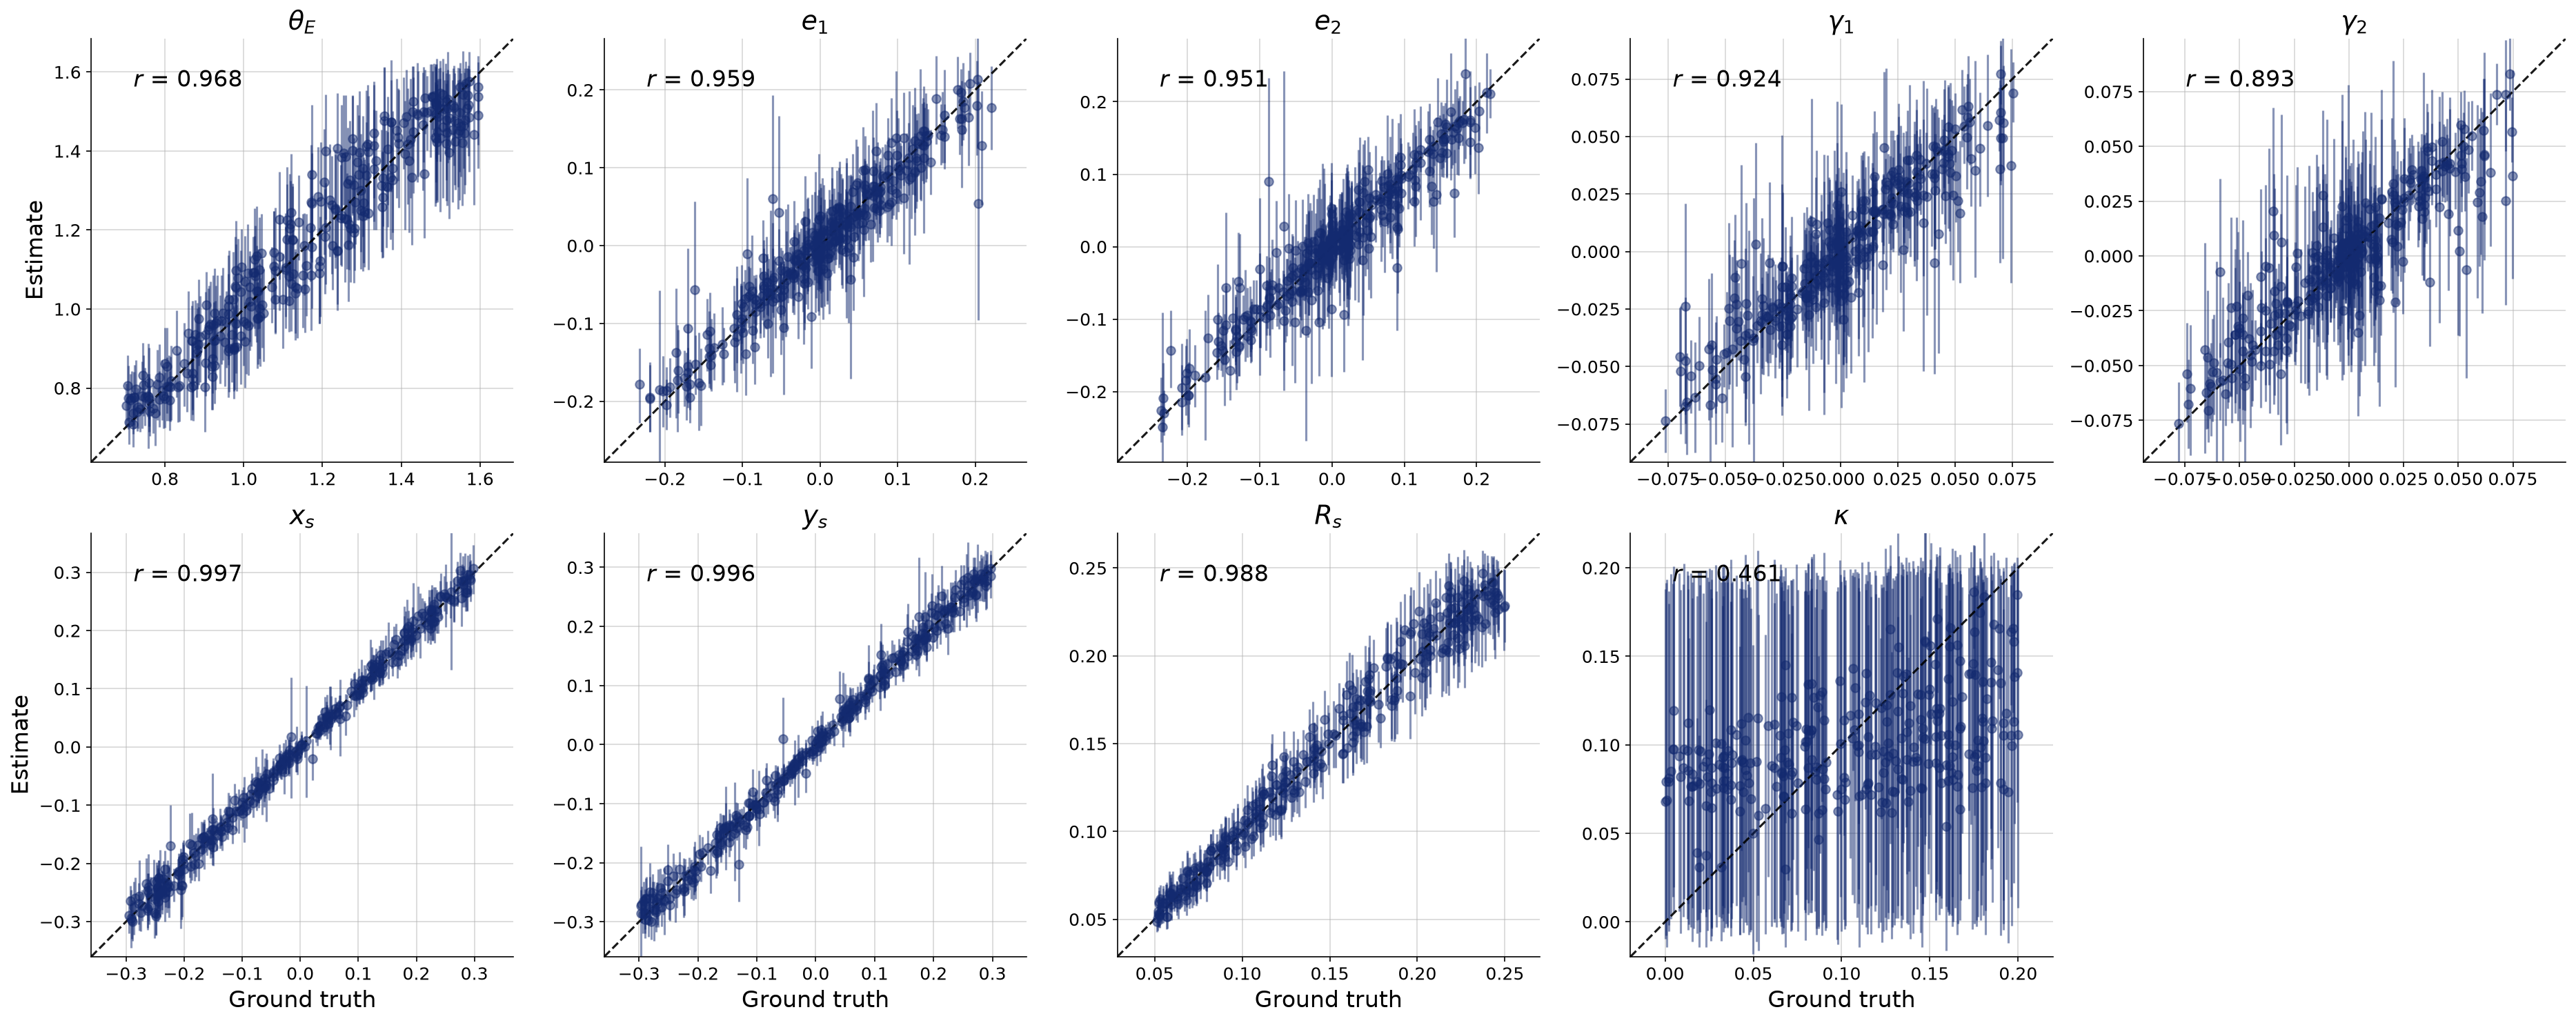
\includegraphics[width=\textwidth]{recovery_kappa.png}
\caption{\textbf{Recovery for the 9-parameter model.} Compare with
Figure~\ref{fig:recovery}. The new $\kappa$ panel (bottom right) is a flat cloud:
estimates hover near the prior average whatever the truth is, with error bars
spanning nearly the whole prior --- the network says ``I don't know''.
Meanwhile the $\theta_E$ panel has visibly widened ($R^2$: $1.00 \to 0.94$);
every other panel is unchanged.}
\label{fig:recovery-kappa}
\end{figure}

Three quantitative signatures, all exactly as theory demands:
\begin{enumerate}
  \item \textbf{$\kappa$ stays unknown.} Prior spread 0.058 $\to$ average
  posterior spread 0.048: a contraction of only 16\%. One image teaches the
  network almost nothing about $\kappa$ --- correctly.
  \item \textbf{The degeneracy direction is discovered.} Within each individual
  posterior, $\kappa$ and $\theta_E$ are correlated at $-0.96$: the network
  learned the precise trade-off (more mass sheet $\Leftrightarrow$ smaller
  intrinsic Einstein radius) that the lens equations predict. Nobody told it.
  And this correlation \emph{sharpened} as our data improved ($-0.83$ in the
  noisy pilot $\to$ $-0.96$ now) --- a sharper posterior hugs the ridge more
  tightly.
  \item \textbf{The damage is surgical.} Only $\theta_E$ pays for the ambiguity
  ($R^2$ $1.00 \to 0.94$); all seven other parameters are untouched. The
  degeneracy couples $\kappa$ to the mass --- and to nothing else.
\end{enumerate}

\begin{figure}[H]
\centering
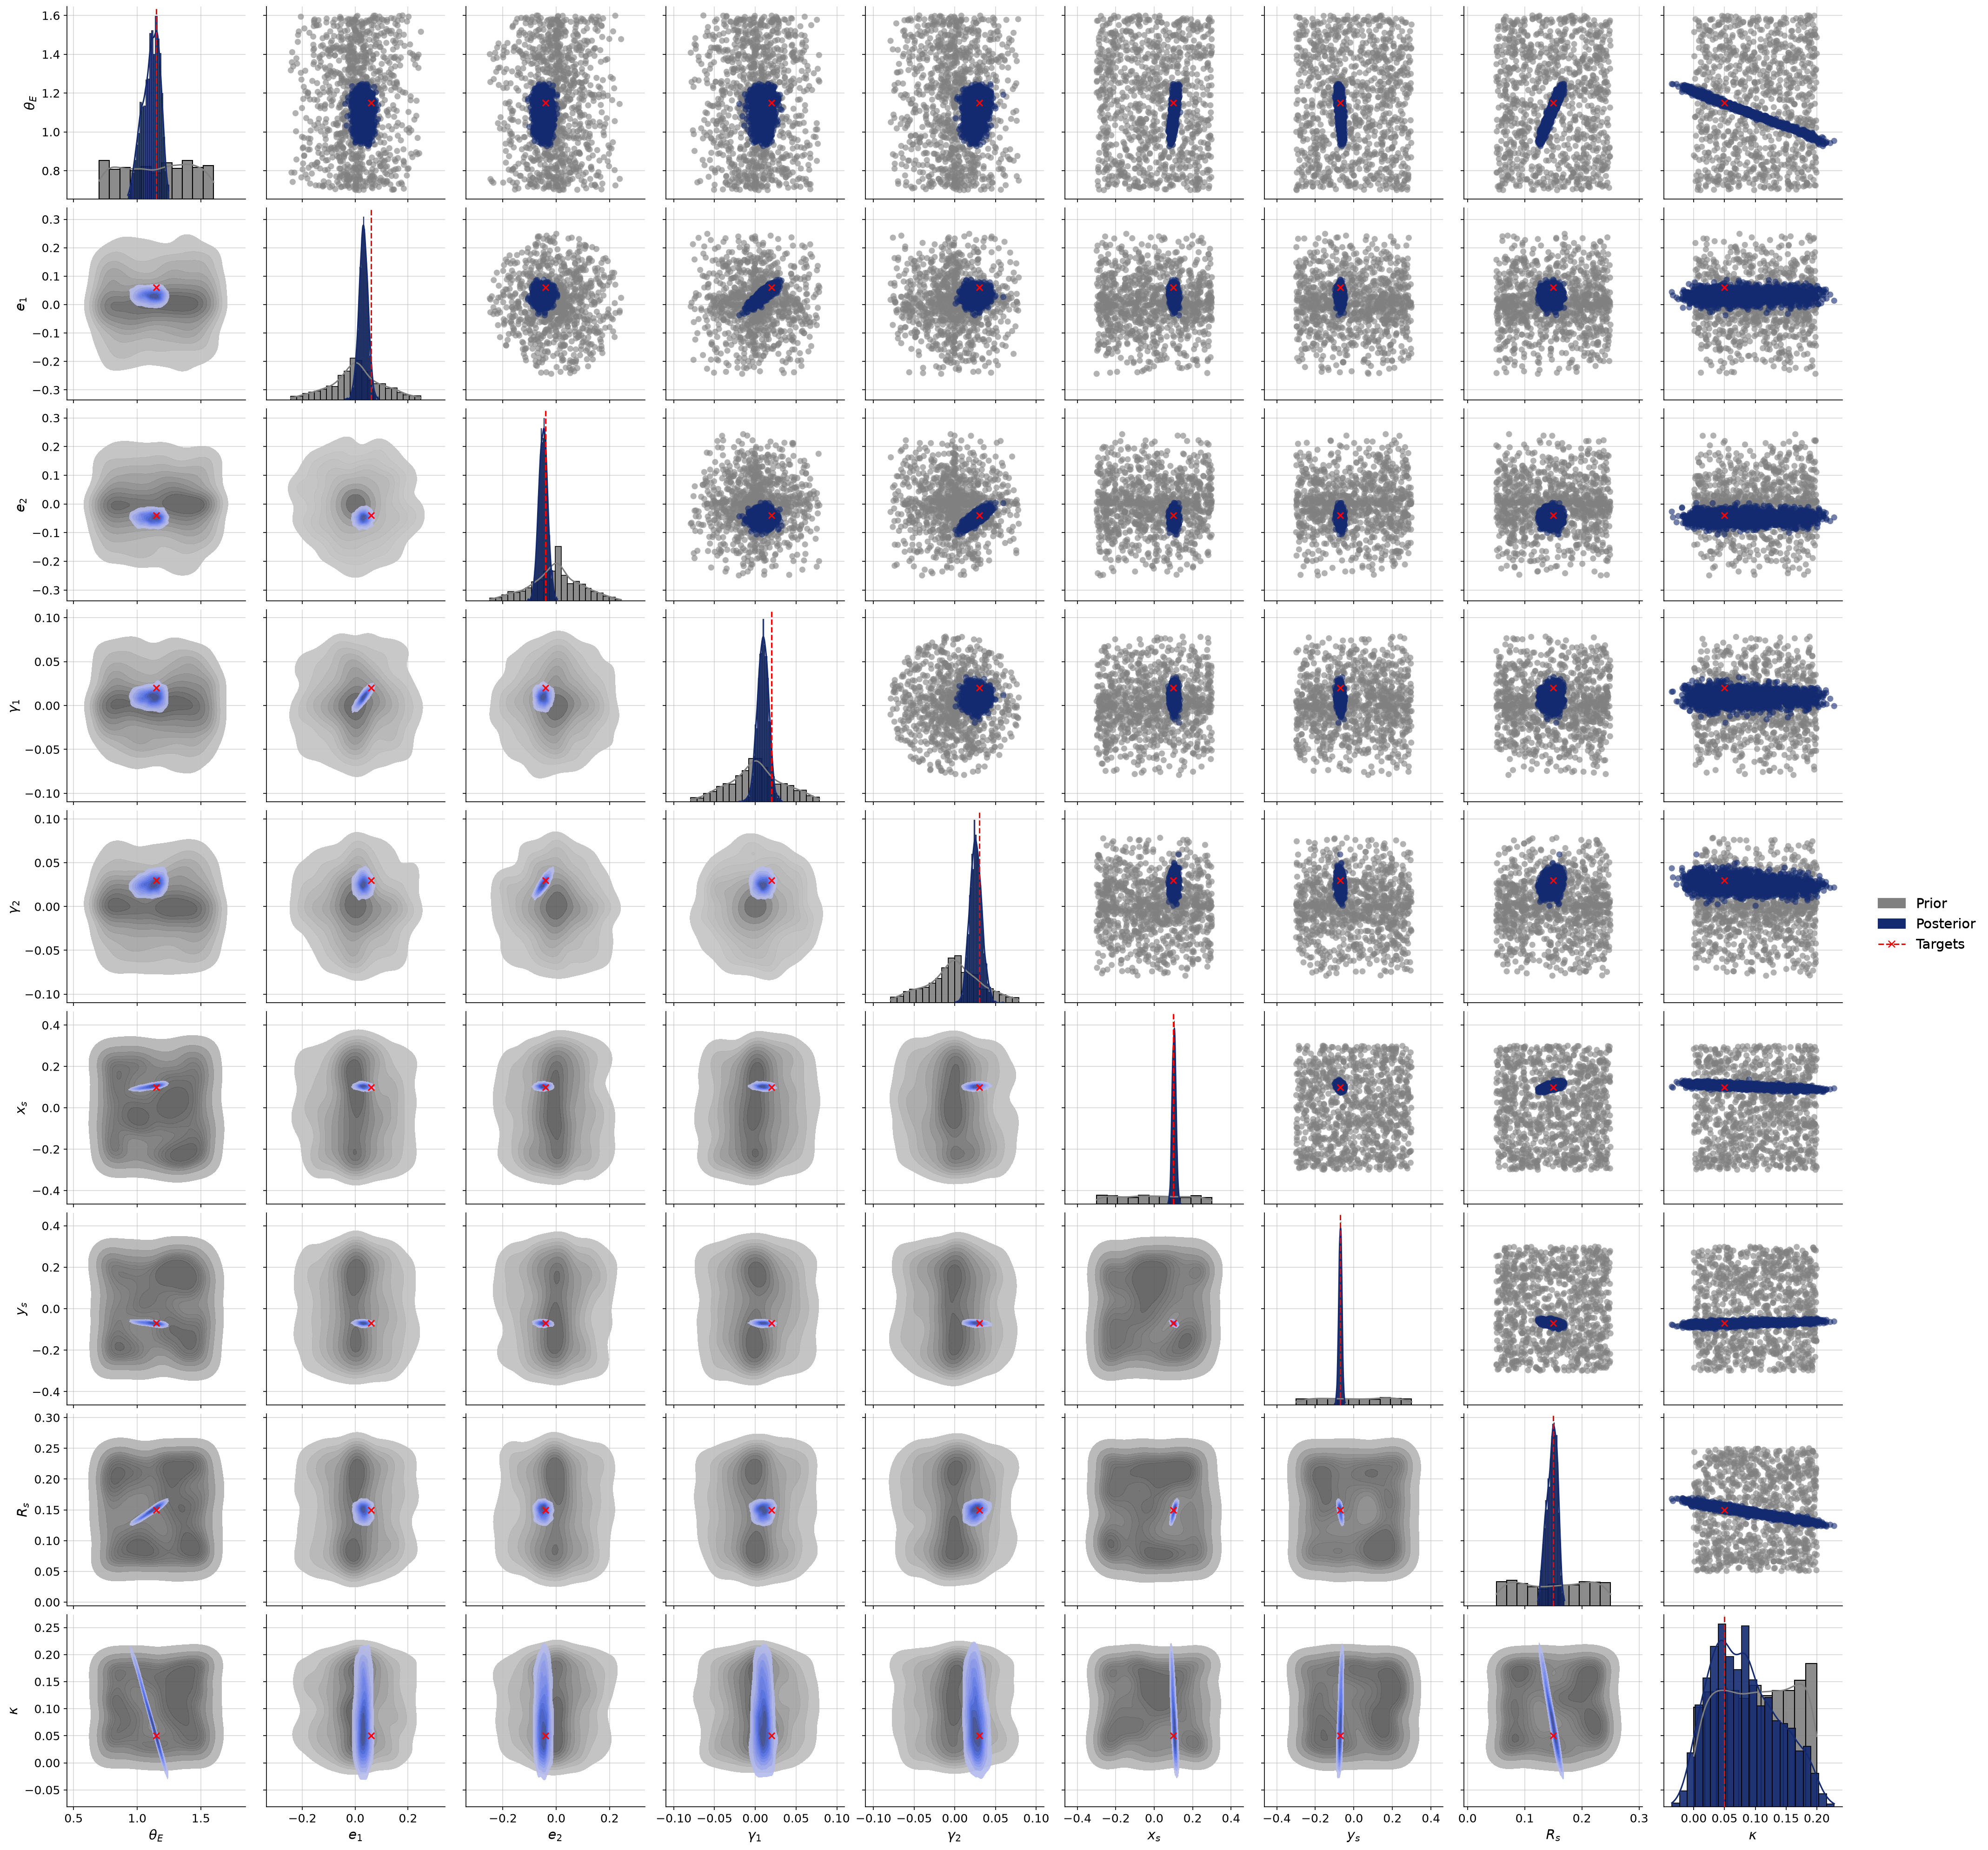
\includegraphics[width=0.95\textwidth]{inference_pairs_kappa.png}
\caption{\textbf{The corner plot with $\kappa$, for the same fiducial system.}
Look at two places. The $\kappa$ diagonal panel: the blue posterior is nearly as
wide as the grey prior --- honest ignorance. The $(\kappa, \theta_E)$ panel: the
posterior is a thin \emph{tilted} ridge --- the degeneracy line itself, drawn by
the network. Compare $\theta_E$'s width here ($\pm 0.065$) with the 8-parameter
fit of the same image ($\pm 0.008$): the unmeasurable mass sheet inflates the
mass uncertainty by a factor $\sim$8, exactly as it must.}
\label{fig:corner-kappa}
\end{figure}

\begin{keyidea}
The network \emph{rediscovered a theorem of gravitational lensing} purely from
simulated examples. For us this is the strongest evidence in the whole project
that the learned posteriors are physically meaningful --- they don't just fit
numbers, they encode the structure of the theory.
\end{keyidea}

% =========================================================================
\section{Everything at a glance}

\begin{center}
\begin{tabular}{p{5.2cm}p{4.2cm}p{5.4cm}}
\toprule
\textbf{Question} & \textbf{Plot that answers it} & \textbf{Our answer} \\
\midrule
Can it recover the parameters? & recovery & $r = 0.999$ for mass/position/size; $0.96$--$0.97$ shape; $0.90$--$0.93$ shear \\
Are the error bars honest? & SBC rank-ECDF & Yes for shape/shear; slightly too cautious (never overconfident) for the rest \\
How much does one image teach? & contraction/z-score & Nearly everything about morphology; honestly partial about shear \\
Does the posterior regenerate the data? & posterior predictive & Yes, down to the bright knots \\
Does it respect known physics? & $\kappa$ diagnostics & Mass-sheet degeneracy reproduced: $\kappa$ unknown, corr$(\kappa,\theta_E) = -0.96$ \\
How fast is it? & --- & Simulate 52k images: $\sim$1 min; train: $\sim$2 h once; infer: milliseconds per lens \\
\bottomrule
\end{tabular}
\end{center}

\section{Glossary}

\begin{description}
  \item[Prior] What you consider plausible before seeing data.
  \item[Likelihood] How probable the observed data is for given parameters ---
  here defined implicitly by the simulator.
  \item[Posterior] Updated beliefs after seeing the data; the full answer,
  including uncertainties and correlations.
  \item[Amortized inference] Train a network once on simulations; afterwards any
  new observation is analysed in milliseconds.
  \item[Summary network] The CNN that compresses each $64{\times}64$ image into
  48 informative numbers.
  \item[Normalizing flow / coupling flow] An invertible network that warps simple
  Gaussian noise into the posterior distribution --- and can therefore both sample
  from it and score it.
  \item[Overfitting] Memorizing the training set instead of learning the pattern;
  detected by a rising validation loss.
  \item[SBC (simulation-based calibration)] The rank-uniformity test of whether
  credible intervals have their claimed coverage.
  \item[Underconfident / overconfident] Error bars too wide (safe) / too narrow
  (dangerous).
  \item[Posterior contraction] How much narrower the posterior is than the prior
  --- the information gained from the data.
  \item[Einstein radius $\theta_E$] The angular radius of the ring; the lensing
  measure of the lens mass.
  \item[External shear $\gamma$] The gentle extra stretch from the gravity of
  neighbouring structures.
  \item[External convergence $\kappa$ / mass-sheet degeneracy] A uniform mass
  sheet that provably cannot be measured from one image; our built-in honesty
  test.
\end{description}

\vspace{1em}
\noindent\textit{Companion documents: the formal write-up is
\texttt{report/report.pdf}; per-run numbers are in \texttt{RESULTS.md}; the
short markdown version of this guide is \texttt{EXPLANATION.md}.}

\end{document}
